% !TeX program = xelatex
\documentclass[a4paper,10pt]{article}

% ============================================================================
% ១. កញ្ចប់បណ្ណាល័យ និងការកំណត់ទំព័រ (Packages & Page Setup — តាមគំរូ ls_plan.tex)
% ============================================================================
\usepackage[a4paper, left=0.95cm, right=0.95cm, top=0.85cm, bottom=0.92cm, footskip=0.52cm]{geometry}
\usepackage{amsmath}
\usepackage{unicode-math}
\usepackage{fontspec}
\usepackage{longtable, array, multirow, colortbl}
\usepackage[table]{xcolor}
\usepackage{enumitem}
\usepackage{pifont}
\usepackage{fancyhdr}
\usepackage{tikz}
\usetikzlibrary{calc, arrows.meta, decorations.pathreplacing, patterns, positioning, babel}

\makeatletter
\let\@expl@@@mark@update@singlecol@structures@@\relax
\makeatother

% --- ប្រព័ន្ធស្វែងរកទីតាំងពុម្ពអក្សរស្វ័យប្រវត្តិ (Windows Local + Cloud Repo fonts/) ---
\providecommand{\NGSFindFonts}{%
  \IfFileExists{C:/Windows/Fonts/cambria.ttc}{%
    \def\NGSSysPath{C:/Windows/Fonts/}%
    \def\NGSUserPath{C:/Users/KIT/AppData/Local/Microsoft/Windows/Fonts/}%
  }{%
    \IfFileExists{./fonts/KhmerOSsiemreap.ttf}{\def\NGSSysPath{./fonts/}\def\NGSUserPath{./fonts/}}{%
    \IfFileExists{../fonts/KhmerOSsiemreap.ttf}{\def\NGSSysPath{../fonts/}\def\NGSUserPath{../fonts/}}{%
    \IfFileExists{../../fonts/KhmerOSsiemreap.ttf}{\def\NGSSysPath{../../fonts/}\def\NGSUserPath{../../fonts/}}{%
    \IfFileExists{../../../fonts/KhmerOSsiemreap.ttf}{\def\NGSSysPath{../../../fonts/}\def\NGSUserPath{../../../fonts/}}{%
    \IfFileExists{../../../../fonts/KhmerOSsiemreap.ttf}{\def\NGSSysPath{../../../../fonts/}\def\NGSUserPath{../../../../fonts/}}{%
    \IfFileExists{../../../../../fonts/KhmerOSsiemreap.ttf}{\def\NGSSysPath{../../../../../fonts/}\def\NGSUserPath{../../../../../fonts/}}{%
    \IfFileExists{../../../../../../fonts/KhmerOSsiemreap.ttf}{\def\NGSSysPath{../../../../../../fonts/}\def\NGSUserPath{../../../../../../fonts/}}{%
      \def\NGSSysPath{../../../../../../../fonts/}\def\NGSUserPath{../../../../../../../fonts/}%
    }}}}}}}%
  }%
}
\NGSFindFonts

% ============================================================================
% ២. កំណត់ពុម្ពអក្សរ (Fonts — តាមគំរូ ls_plan.tex)
% ============================================================================
\setmathfont[Path={\NGSSysPath}, FontIndex=1, Scale=1.02]{cambria.ttc}
\defaultfontfeatures{Ligatures=TeX}

\setmainfont[
  Path={\NGSUserPath},
  Extension=.ttf,
  Script=Khmer,
  BoldFont={KhmerOSsiemreap},
  BoldFeatures={FakeBold=1.8},
  ItalicFont={KhmerOSsiemreap},
  ItalicFeatures={FakeSlant=0.25},
  BoldItalicFont={KhmerOSsiemreap},
  BoldItalicFeatures={FakeBold=1.8, FakeSlant=0.25}
]{KhmerOSsiemreap}

\newfontfamily\muol[Path={\NGSUserPath}, Extension=.ttf, Script=Khmer]{KhmerOSmuollight}
\newfontfamily\Tacteing[Path={\NGSUserPath}, Extension=.TTF]{TACTENG}
\newfontfamily\TimesEn[Path={\NGSSysPath}, Extension=.ttf, BoldFont={timesbd}, ItalicFont={timesi}, BoldItalicFont={timesbi}]{times}
\newfontfamily\CalibriFont[Path={\NGSSysPath}, Extension=.ttf]{calibri}
\newfontfamily\CourierCirc[Path={\NGSSysPath}, Extension=.ttf]{cour}

\XeTeXlinebreaklocale "km"
\XeTeXlinebreakskip = 0pt plus 1pt minus 0.1pt

% ============================================================================
% ៣. ពណ៌ និងការតុបតែង (Colors & Styles)
% ============================================================================
\definecolor{stepbg}{HTML}{D9D9D9}
\definecolor{headgray}{HTML}{E6E6E6}
\definecolor{emphred}{HTML}{C00000}

\pagestyle{fancy}
\fancyhf{}
\renewcommand{\headrulewidth}{0pt}
\fancyfoot[R]{\CalibriFont\fontsize{9pt}{11pt}\selectfont\thepage}

\setlength{\parindent}{0pt}
\setlength{\parskip}{0pt}
\setlength{\tabcolsep}{4.5pt}
\setlength{\LTpre}{2pt}
\setlength{\LTpost}{2pt}

\newcolumntype{L}[1]{>{\raggedright\arraybackslash}p{#1}}
\newcolumntype{C}[1]{>{\centering\arraybackslash}p{#1}}

% ============================================================================
% ៤. ពាក្យបញ្ជាជំនួយ (Helper Macros)
% ============================================================================
\newcommand{\en}[1]{{\TimesEn #1}}
\newcommand{\enbf}[1]{{\TimesEn\bfseries #1}}
\newcommand{\khmflourish}{{\Tacteing\fontsize{15pt}{15pt}\selectfont 3}}
\newcommand{\wcirc}{{\CourierCirc\fontsize{9.5pt}{11pt}\selectfont o}}
\newcommand{\ditem}{{\fontsize{7.5pt}{10pt}\selectfont\ding{117}}\ }
\newcommand{\fiveE}[1]{\textcolor{emphred}{\CalibriFont\bfseries #1}}
\newcommand{\redsub}[1]{\textcolor{emphred}{#1}}
\newcommand{\timenote}[1]{\textcolor{emphred}{\textit{#1}}}
\newcommand{\stepheader}[1]{\multicolumn{3}{|c|}{\cellcolor{stepbg}\muol #1} \\ \hline}
\newcommand{\cfig}[1]{{\centering\vspace{3pt}#1\vspace{3pt}\par}}
\newcommand{\cnum}[1]{\mbox{\fontsize{10.5pt}{12pt}\selectfont\ding{\numexpr181+#1\relax}}}
\newcommand{\unit}[1]{\,\text{\en{#1}}}
\newcommand{\graybox}[1]{\colorbox{headgray}{\strut #1}}

% ============================================================================
% ៥. រូបភាព TikZ ស-ខ្មៅ សម្រាប់បង្រៀនលើក្ដារខៀន និងសន្លឹកកិច្ចការ (B&W Diagrams)
% ============================================================================

% ១. E1 Engage: អន្ទាក់លេខសូន្យ (0) និងចុងដែនស្លាកលេខផ្ទះគូ 72 < n <= 90
\newcommand{\figEngageWNOneOne}{%
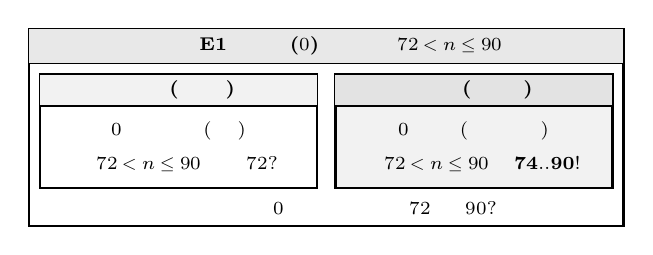
\begin{tikzpicture}[x=1cm, y=1cm, every node/.style={font=\fontsize{6.7pt}{8.6pt}\selectfont, text=black}]
  \draw[black, line width=0.9pt] (0,0) rectangle (7.55,2.50);
  \fill[gray!18] (0,2.06) rectangle (7.55,2.50);
  \draw[black, line width=0.6pt] (0,2.06) -- (7.55,2.06);
  \node at (3.775,2.28) {\textbf{បេសកកម្ម \en{E1}៖ លេខសូន្យ ($0$) និងលេខផ្ទះគូ $72 < n \le 90$}};

  % Left: Student A
  \draw[black, line width=0.8pt] (0.14,0.48) rectangle (3.66,1.92);
  \fill[gray!10] (0.14,1.52) rectangle (3.66,1.92);
  \draw[black, line width=0.5pt] (0.14,1.52) -- (3.66,1.52);
  \node at (1.90,1.72) {\textbf{សិស្ស ក (ភាន់ច្រឡំ)}};
  \node at (1.90,1.20) {$0$ ជាគត់ធម្មជាតិ (មិនគូ)};
  \node at (1.90,0.78) {គូ $72 < n \le 90$ យកទាំង $72$?};

  % Right: Student B
  \draw[black, line width=0.95pt, fill=gray!10] (3.89,0.48) rectangle (7.41,1.92);
  \fill[gray!22] (3.89,1.52) rectangle (7.41,1.92);
  \draw[black, line width=0.55pt] (3.89,1.52) -- (7.41,1.52);
  \node at (5.65,1.72) {\textbf{សិស្ស ខ (តាមនិយមន័យ)}};
  \node at (5.65,1.20) {$0$ ជាគត់គូ (មិនមែនធម្មជាតិ)};
  \node at (5.65,0.78) {គូ $72 < n \le 90$ គឺ $\mathbf{74..90}$!};

  \node at (3.775,0.22) {\textbf{សំណួរគន្លឹះ៖} ហេតុអ្វី $0$ ជាចំនួនគត់គូ ហើយមិនយក $72$ តែយក $90$?};
\end{tikzpicture}}

% ២. E2 Explore: បន្ទាត់ចំនួននៃលំហាត់គំរូ ១ (ទំ.២៖ ធំជាង 4 និងតូចជាង 11)
\newcommand{\figNumberLineWNOneOne}{%
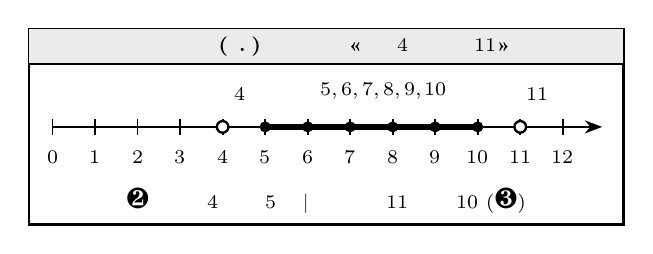
\begin{tikzpicture}[x=1cm, y=1cm, every node/.style={font=\scriptsize, text=black}]
  \draw[black, line width=0.9pt] (0,0) rectangle (7.55,2.48);
  \fill[gray!16] (0,2.04) rectangle (7.55,2.48);
  \draw[black, line width=0.6pt] (0,2.04) -- (7.55,2.04);
  \node at (3.775,2.26) {\textbf{លំហាត់គំរូ ១ (ទំ.២)៖ បន្ទាត់ចំនួន «ធំជាង $4$ និងតូចជាង $11$»}};

  % Number line 0 to 12
  \draw[-{Stealth[length=2.2mm]}, black, line width=0.85pt] (0.30,1.24) -- (7.28,1.24);
  % Highlight thick segment from 5 to 10
  \draw[black, line width=2.2pt] (3.00,1.24) -- (5.70,1.24);

  \foreach \i in {0,1,2,3,4,5,6,7,8,9,10,11,12} {
    \pgfmathsetmacro{\xx}{0.30 + \i*0.54}
    \draw[black, line width=0.65pt] (\xx,1.14) -- (\xx,1.34);
    \node at (\xx,0.86) {$\i$};
  }
  % Open circles at 4 and 11, solid dots on 5..10
  \draw[black, fill=white, line width=0.85pt] (2.46,1.24) circle (2.1pt);
  \draw[black, fill=white, line width=0.85pt] (6.24,1.24) circle (2.1pt);
  \foreach \k in {5,6,7,8,9,10} {
    \pgfmathsetmacro{\xk}{0.30 + \k*0.54}
    \fill[black] (\xk,1.24) circle (2.0pt);
  }
  \node at (2.46,1.66) {មិនយក $4$};
  \node at (4.35,1.70) {\textbf{យក៖ $5, 6, 7, 8, 9, 10$}};
  \node at (6.24,1.66) {មិនយក $11$};
  \node at (3.775,0.30) {\cnum{2} ខាងស្ដាំ $4$ ចាប់ពី $5$ $\quad|\quad$ ខាងឆ្វេង $11$ ចាប់ពី $10$ (\cnum{3})};
\end{tikzpicture}}

% ៣. E3 Explain: ផែនទីសំណុំចំនួនគត់ និងការបែងចែកគូ-សេស
\newcommand{\figSummaryWNOneOne}{%
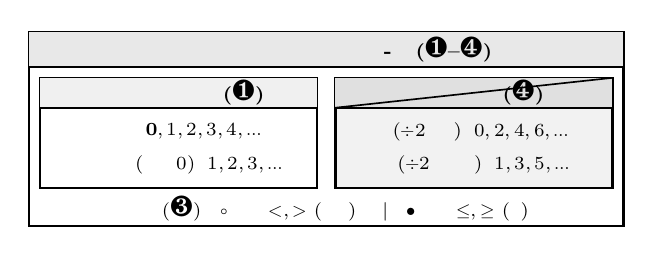
\begin{tikzpicture}[x=1cm, y=1cm, every node/.style={font=\fontsize{6.7pt}{8.6pt}\selectfont, text=black}]
  \draw[black, line width=0.9pt] (0,0) rectangle (7.55,2.46);
  \fill[gray!18] (0,2.02) rectangle (7.55,2.46);
  \draw[black, line width=0.6pt] (0,2.02) -- (7.55,2.02);
  \node at (3.775,2.24) {\textbf{សង្ខេបរចនាសម្ព័ន្ធចំនួនគត់ លំដាប់ និងភាពគូ-សេស (\cnum{1}--\cnum{4})}};

  % Left box: Whole vs Natural
  \draw[black, line width=0.8pt] (0.14,0.48) rectangle (3.66,1.88);
  \fill[gray!12] (0.14,1.50) rectangle (3.66,1.88);
  \draw[black, line width=0.55pt] (0.14,1.50) -- (3.66,1.50);
  \node at (1.90,1.69) {\textbf{ចំនួនគត់ និងគត់ធម្មជាតិ (\cnum{1})}};
  \node at (1.90,1.20) {ចំនួនគត់៖ $\mathbf{0}, 1, 2, 3, 4, \dots$};
  \node at (1.90,0.78) {គត់ធម្មជាតិ (គ្មាន $0$)៖ $1, 2, 3, \dots$};

  % Right box: Even vs Odd
  \draw[black, line width=0.95pt, fill=gray!10] (3.89,0.48) rectangle (7.41,1.88);
  \fill[gray!24] (3.89,1.50) rectangle (7.41,1.88);
  \draw[black, line width=0.6pt] (3.89,1.50) -- (7.41,1.88);
  \draw[black, line width=0.6pt] (3.89,1.50) -- (7.41,1.50);
  \node at (5.65,1.69) {\textbf{ចំនួនគត់គូ និងសេស (\cnum{4})}};
  \node at (5.65,1.20) {គូ ($\div 2$ ដាច់)៖ $0, 2, 4, 6, \dots$};
  \node at (5.65,0.78) {សេស ($\div 2$ មិនដាច់)៖ $1, 3, 5, \dots$};

  \node at (3.775,0.22) {ចុងដែន (\cnum{3})៖ \ $\circ$ ចំពោះ $<, >$ (មិនយក) \quad|\quad $\bullet$ ចំពោះ $\le, \ge$ (យក)};
\end{tikzpicture}}

% ៤. E4 Elaborate: ដើមឈើរៀបឆ្លាស់លេខ 3, 4, 5 (លំហាត់គំរូ ២ ទំ.២)
\newcommand{\figPermTreeWNOneOne}{%
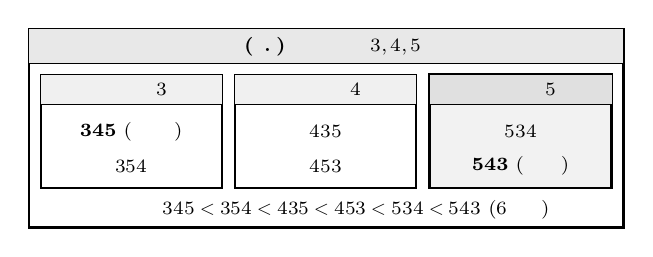
\begin{tikzpicture}[x=1cm, y=1cm, every node/.style={font=\fontsize{6.8pt}{8.8pt}\selectfont, text=black}]
  \draw[black, line width=0.9pt] (0,0) rectangle (7.55,2.52);
  \fill[gray!18] (0,2.08) rectangle (7.55,2.52);
  \draw[black, line width=0.6pt] (0,2.08) -- (7.55,2.08);
  \node at (3.775,2.30) {\textbf{លំហាត់គំរូ ២ (ទំ.២)៖ រៀបឆ្លាស់លេខ $3, 4, 5$ តាមខ្ទង់រយ}};

  % Three column boxes for hundreds digit 3, 4, 5
  \draw[black, line width=0.8pt] (0.15,0.50) rectangle (2.45,1.94);
  \fill[gray!12] (0.15,1.56) rectangle (2.45,1.94);
  \draw[black, line width=0.5pt] (0.15,1.56) -- (2.45,1.56);
  \node at (1.30,1.75) {\textbf{ខ្ទង់រយលេខ $3$}};
  \node at (1.30,1.22) {$\mathbf{345}$ (តូចបំផុត)};
  \node at (1.30,0.78) {$354$};

  \draw[black, line width=0.8pt] (2.62,0.50) rectangle (4.92,1.94);
  \fill[gray!12] (2.62,1.56) rectangle (4.92,1.94);
  \draw[black, line width=0.5pt] (2.62,1.56) -- (4.92,1.56);
  \node at (3.77,1.75) {\textbf{ខ្ទង់រយលេខ $4$}};
  \node at (3.77,1.22) {$435$};
  \node at (3.77,0.78) {$453$};

  \draw[black, line width=0.95pt, fill=gray!10] (5.09,0.50) rectangle (7.40,1.94);
  \fill[gray!24] (5.09,1.56) rectangle (7.40,1.94);
  \draw[black, line width=0.6pt] (5.09,1.56) -- (7.40,1.56);
  \node at (6.245,1.75) {\textbf{ខ្ទង់រយលេខ $5$}};
  \node at (6.245,1.22) {$534$};
  \node at (6.245,0.78) {$\mathbf{543}$ (ធំបំផុត)};

  \node at (3.775,0.22) {លំដាប់កើន៖ $345 < 354 < 435 < 453 < 534 < 543$ ($6$ ចំនួន)};
\end{tikzpicture}}

% ៥. E5 Evaluate: ជម្រើសវិនិច្ឆ័យ A-D (ចំនួនគត់សេស n ដែល 49 < n <= 57)
\newcommand{\figExitWNOneOne}{%
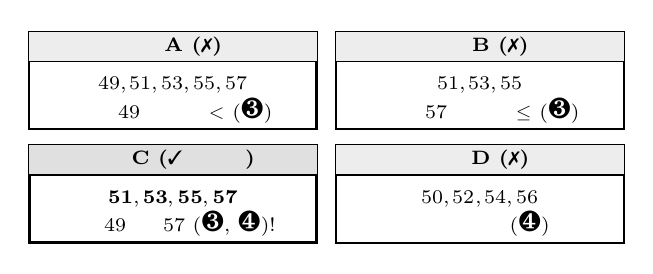
\begin{tikzpicture}[x=1cm, y=1cm, every node/.style={font=\scriptsize, text=black}]
  % Choice A
  \draw[black, line width=0.8pt] (0,1.44) rectangle (3.65,2.68);
  \fill[gray!14] (0,2.30) rectangle (3.65,2.68);
  \draw[black, line width=0.5pt] (0,2.30) -- (3.65,2.30);
  \node at (1.825,2.49) {\textbf{ជម្រើស \en{A} (\ding{55})}};
  \node at (1.825,2.00) {$49, 51, 53, 55, 57$};
  \node at (1.825,1.68) {ច្រឡំយក $49$ ត្រង់សញ្ញា $<$ (\cnum{3})};

  % Choice B
  \draw[black, line width=0.8pt] (3.90,1.44) rectangle (7.55,2.68);
  \fill[gray!14] (3.90,2.30) rectangle (7.55,2.68);
  \draw[black, line width=0.5pt] (3.90,2.30) -- (7.55,2.30);
  \node at (5.725,2.49) {\textbf{ជម្រើស \en{B} (\ding{55})}};
  \node at (5.725,2.00) {$51, 53, 55$};
  \node at (5.725,1.68) {ភ្លេចយក $57$ ត្រង់សញ្ញា $\le$ (\cnum{3})};

  % Choice C (Correct)
  \draw[black, line width=1.05pt] (0,0) rectangle (3.65,1.24);
  \fill[gray!24] (0,0.86) rectangle (3.65,1.24);
  \draw[black, line width=0.6pt] (0,0.86) -- (3.65,0.86);
  \node at (1.825,1.05) {\textbf{ជម្រើស \en{C} (\ding{51} ត្រឹមត្រូវ)}};
  \node at (1.825,0.56) {$\mathbf{51, 53, 55, 57}$};
  \node at (1.825,0.24) {មិនយក $49$ តែយក $57$ (\cnum{3}, \cnum{4})!};

  % Choice D
  \draw[black, line width=0.8pt] (3.90,0) rectangle (7.55,1.24);
  \fill[gray!14] (3.90,0.86) rectangle (7.55,1.24);
  \draw[black, line width=0.5pt] (3.90,0.86) -- (7.55,0.86);
  \node at (5.725,1.05) {\textbf{ជម្រើស \en{D} (\ding{55})}};
  \node at (5.725,0.56) {$50, 52, 54, 56$};
  \node at (5.725,0.24) {ច្រឡំយកចំនួនគត់គូ (\cnum{4})};
\end{tikzpicture}}

\begin{document}
\fontsize{10pt}{15.2pt}\selectfont

% ============================================================================
% ក្បាលរដ្ឋបាល (Administrative Header — តាមគំរូ ls_plan.tex)
% ============================================================================
{\centering
  {\muol\fontsize{11pt}{16pt}\selectfont ព្រះរាជាណាចក្រកម្ពុជា\par}
  {\muol\fontsize{11pt}{16pt}\selectfont ជាតិ សាសនា ព្រះមហាក្សត្រ\par}
  \vspace{-3pt}{\khmflourish\par}
}

\vspace{1pt}
{\muol\fontsize{10pt}{15.5pt}\selectfont
មន្ទីរអប់រំ យុវជន និងកីឡា ខេត្តកំពង់ធំ\par
ការិយាល័យអប់រំ យុវជន និងកីឡា ស្រុកកំពង់ស្វាយ\par
អនុវិទ្យាល័យព្រះក្រសាំង\par}

\vspace{2pt}
{\centering{\muol\fontsize{11.5pt}{17pt}\selectfont កិច្ចតែងការបង្រៀន\par}}
\vspace{2pt}

% --- ព័ត៌មានទូទៅ ---
{\hspace*{2.8cm}\renewcommand{\arraystretch}{1.08}
\begin{tabular}{@{}l@{\hspace{0.35cm}}p{2.9cm}@{\hspace{0.15cm}}c@{\hspace{0.25cm}}l@{}}
  - & មុខវិជ្ជា & : & គណិតវិទ្យា ថ្នាក់ទី៧ (ពីជគណិត) \\
  - & ចំណងជើងមេរៀន & : & មេរៀនទី១៖ ចំនួនគត់ \\
  - & ចំណងជើងរង & : & ១. សញ្ញាណចំនួនគត់ ២. លំដាប់ និង ៣. ចំនួនគត់គូនិងសេស (ទំ.១--៣) \\
  - & រយៈពេល & : & ១ ម៉ោងសិក្សា (៥០ នាទី) \\
  - & បង្រៀនដោយ & : & ហុក ប៊ុនថែន \\
  - & កាលបរិច្ឆេទ & : & ថ្ងៃអង្គារ ទី៣ ខែវិច្ឆិកា ឆ្នាំ២០២៦ \\
\end{tabular}\par}

\vspace{2pt}

% --- I. វត្ថុបំណង ---
{\muol\fontsize{10pt}{15.5pt}\selectfont \enbf{I.} វត្ថុបំណង\par}
\vspace{1pt}
{\renewcommand{\arraystretch}{1.10}
\begin{tabular}{@{}p{0.55cm}@{}p{2.35cm}@{\hspace{0.15cm}}c@{\hspace{0.25cm}}p{14.95cm}@{}}
  \hfill\wcirc\hspace{0.2cm} & វិជ្ជាសម្បទា & : & សិស្សប្រាប់បានពីលេខហ៊ិនឌូអារ៉ាប់ទាំងដប់ ($0$--$9$) ភាពខុសគ្នារវាងចំនួនគត់ ($0, 1, 2, \dots$) និងចំនួនគត់ធម្មជាតិ ($1, 2, 3, \dots$) វិធានលំដាប់លើបន្ទាត់ចំនួន និងនិយមន័យចំនួនគត់គូ/សេសបានត្រឹមត្រូវ ។ \\
  \hfill\wcirc\hspace{0.2cm} & បំណិនសម្បទា & : & សិស្សតាងនិងកំណត់ផ្នែកនៃបន្ទាត់ចំនួន រៀបឆ្លាស់តួលេខរកចំនួនធំបំផុត/តូចបំផុត និងកំណត់សំណុំចំនួនគត់គូឬសេសក្នុងចន្លោះវិសមភាព ($<, \le$) លើសន្លឹកកិច្ចការបានត្រឹមត្រូវ ។ \\
  \hfill\wcirc\hspace{0.2cm} & ចរិយាសម្បទា & : & សិស្សមានទម្លាប់ពិនិត្យលក្ខខណ្ឌចុងដែនដោយផ្ចិតផ្ចង់ ចេះសហការពិភាក្សាក្នុងក្រុមតូច និងប្រើប្រាស់លំដាប់លេខរៀងក្នុងជីវភាពរស់នៅប្រចាំថ្ងៃប្រកបដោយសណ្ដាប់ធ្នាប់ ។ \\
\end{tabular}\par}

\vspace{2pt}

% --- II. សម្ភារៈឧបទេស ---
{\muol\fontsize{10pt}{15.5pt}\selectfont \enbf{II.} សម្ភារៈឧបទេស\par}
\vspace{1pt}
\hspace*{0.55cm}$\bullet$\ សៀវភៅសិក្សាគោលថ្នាក់ទី៧ (ទំ.១--៣ និងទំ.១៤) ក្ដារខៀន ដីស/ហ្វឺត បន្ទាត់ត្រង់ និង\textbf{សន្លឹកកិច្ចការសិស្សបំពេញចន្លោះ ស-ខ្មៅ} (កូដ \en{WN11} ទំព័រ ១--២ សម្រាប់សិស្ស និងទំព័រ ៣ ប្លង់ក្ដារខៀន/ចម្លើយគ្រូ — គ្មានប្រើ \en{LCD})\par

\vspace{2pt}

% --- III. វិធីសាស្រ្តបង្រៀន ---
{\muol\fontsize{10pt}{15.5pt}\selectfont \enbf{III.} វិធីសាស្រ្តបង្រៀន\par}
\vspace{1pt}
{\renewcommand{\arraystretch}{1.08}
\begin{tabular}{@{}p{0.55cm}@{}p{2.35cm}@{\hspace{0.15cm}}c@{\hspace{0.25cm}}p{14.95cm}@{}}
  \hfill$\bullet$\hspace{0.2cm} & គោលវិធី & : & សិស្សមជ្ឈមណ្ឌល (សន្លឹកកិច្ចការបំពេញចន្លោះជាគោល + ការពិភាក្សាជាក្រុមតូច ៣ នាក់) \\
  \hfill$\bullet$\hspace{0.2cm} & យុទ្ធវិធីបង្រៀន & : & គំរូស្ថាបនានិយម \en{5Es} រួមបញ្ចូល \textbf{ការប្រៀបធៀបនិយមន័យទល់នឹងរូបារម្មណ៍ (\en{Concept-Definition Contrast})} និង \textbf{ការតាងចុងដែនលើបន្ទាត់ចំនួន ($\circ$ ទល់នឹង $\bullet$)} \\
\end{tabular}\par}

\vspace{2pt}

% --- IV. ដំណើរការបង្រៀន ---
{\muol\fontsize{10pt}{15.5pt}\selectfont \enbf{IV.} ដំណើរការបង្រៀន\par}

{\renewcommand{\arraystretch}{1.15}
\begin{longtable}{|L{5.50cm}|L{7.90cm}|L{4.80cm}|}
\hline
\multicolumn{1}{|c|}{\cellcolor{headgray}\muol សកម្មភាពគ្រូ} &
\multicolumn{1}{c|}{\cellcolor{headgray}\muol ខ្លឹមសារមេរៀន} &
\multicolumn{1}{c|}{\cellcolor{headgray}\muol សកម្មភាពសិស្ស} \\
\hline
\endfirsthead

\hline
\multicolumn{1}{|c|}{\cellcolor{headgray}\muol សកម្មភាពគ្រូ} &
\multicolumn{1}{c|}{\cellcolor{headgray}\muol ខ្លឹមសារមេរៀន} &
\multicolumn{1}{c|}{\cellcolor{headgray}\muol សកម្មភាពសិស្ស} \\
\hline
\endhead

% ==================== ជំហានទី១ (2min) ====================
\stepheader{ជំហានទី១ \enbf{(}រដ្ឋបាលថ្នាក់\enbf{)}}
$\bullet$ ពិនិត្យវត្តមាន អនាម័យ និងសណ្ដាប់ធ្នាប់ថ្នាក់រៀនដើមឆ្នាំសិក្សា \par
$\bullet$ រៀបចំក្រុមតូច ៣ នាក់តាមតុ និងចែក\textbf{សន្លឹកកិច្ចការសិស្ស (\en{WN11} ទំព័រ ១–២)}
&
$\bullet$ រដ្ឋបាលថ្នាក់ អនាម័យ និងវិន័យសិក្សាថ្នាក់ទី៧ \par
$\bullet$ ចែកសន្លឹកកិច្ចការម្នាក់ ១ សន្លឹក សម្រាប់បំពេញតាមដំណាក់កាល \en{E1--E5}
&
$\circ$ ប្រធានថ្នាក់រាយការណ៍វត្តមានសិស្ស \par
$\circ$ ទទួលសន្លឹកកិច្ចការ សរសេរឈ្មោះ និងអង្គុយតាមក្រុម ៣ នាក់ \\
\hline

% ==================== ជំហានទី២ (9min: ពិនិត្យមូលដ្ឋាន <=3m + រំលឹក 3m + E1 3m) ====================
\stepheader{ជំហានទី២ \enbf{(}ពិនិត្យចំណេះដឹងមូលដ្ឋាន \enbf{+} ទំនាក់ទំនងមេរៀនថ្មី\enbf{)}}
\ditem \textbf{ស្ទង់ចំណេះដឹងមូលដ្ឋានដើមឆ្នាំ ($\le\text{\enbf{3\,min}}$)} \par
$\bullet$ ហៅសិស្ស ២ នាក់ឡើងសរសេរជាលេខនូវចំនួន «មួយពាន់ប្រាំបួនរយហាសិបបី» និងប្រាប់តម្លៃតាមខ្ទង់លើក្ដារខៀន
&
{\centering\redsub{ពិនិត្យចំណេះដឹងមូលដ្ឋានពីថ្នាក់ទី៦ (ម៉ោងទី ១ ដើមឆ្នាំ)}\par}
$\bullet$ «មួយពាន់ប្រាំបួនរយហាសិបបី» តាងដោយ $\mathbf{1953}$ \par
$\bullet$ ខ្ទង់ពាន់ $= 1$, ខ្ទង់រយ $= 9$, ខ្ទង់ដប់ $= 5$, និងខ្ទង់រាយ $= 3$
&
$\circ$ សរសេរលេខ $1953$ និងផ្ទៀងតម្លៃតាមខ្ទង់ជាមួយគ្រូ \\[3pt]

\ditem \textbf{រំលឹកមេរៀនទាក់ទង (\enbf{3min})} \par
$\bullet$ សួរ៖ «តើលេខដែលយើងប្រើសរសេរចំនួនសព្វថ្ងៃមានប៉ុន្មានតួ? គឺលេខអ្វីខ្លះ?»
&
{\centering\redsub{រំលឹកតួលេខ និងសញ្ញាប្រៀបធៀប}\par}
$\bullet$ មានលេខដប់តួគឺ៖ $0, 1, 2, 3, 4, 5, 6, 7, 8$ និង $9$
&
$\circ$ ឆ្លើយ៖ «មាន ១០ លេខ គឺពីលេខ $0$ ដល់លេខ $9$!» \\[3pt]

$\bullet$ សួរបន្ត៖ «រវាង $7$ និង $4$ តើមួយណាធំជាង? ចុះសញ្ញា $<$ និង $\le$ ខុសគ្នាដូចម្ដេច?»
&
$\bullet$ $7 > 4$ (ប្រាំពីរធំជាងបួន); សញ្ញា $<$ មិនរាប់បញ្ចូលចុងដែនទេ ឯសញ្ញា $\le$ រាប់បញ្ចូលទាំងតម្លៃស្មើចុងដែន
&
$\circ$ ឆ្លើយប្រៀបធៀបសញ្ញា $>$, $<$ និង $\le$ \\[3pt]

\fiveE{E1 - Engage (3min)} \timenote{(កុំទាន់ផ្ដល់ចម្លើយ)} \par
\ditem \textbf{បេសកកម្មអន្ទាក់លេខសូន្យ និងស្លាកលេខផ្ទះ (សន្លឹកកិច្ចការ \en{E1})} \par
$\bullet$ ឱ្យសិស្សអានប្រអប់ \en{E1} ហើយគូសជ្រើសរើសរវាង\textbf{សិស្ស ក} និង\textbf{សិស្ស ខ}
&
\redsub{បេសកកម្ម \en{E1}៖ លេខសូន្យ ($0$) និងលេខផ្ទះគូ $72 < n \le 90$} \par
$\bullet$ \textbf{សិស្ស ក៖} «$0$ ជាចំនួនគត់ធម្មជាតិ មិនមែនគូទេ ឯគូ $72 < n \le 90$ រាប់ទាំង $72$ ដែរ» \par
$\bullet$ \textbf{សិស្ស ខ៖} «$0$ ជាចំនួនគត់គូ (តែមិនមែនធម្មជាតិ) ឯគូ $72 < n \le 90$ គឺពី $74$ ដល់ $90$»
&
$\circ$ ពិភាក្សាជាគូ និងគូស \ding{51} ក្នុងប្រអប់ \en{E1} លើសន្លឹកកិច្ចការ \\[3pt]

&
\cfig{\figEngageWNOneOne}
& \\
\hline

% ==================== ជំហានទី៣ (17min: E2 11m + E3 6m) ====================
\stepheader{ជំហានទី៣ \enbf{(}ខ្លឹមសារមេរៀនថ្មី\enbf{)}}
\fiveE{E2 - Explore (11min)} \par
$\bullet$ សរសេរចំណងជើង \textbf{មេរៀនទី១៖ ចំនួនគត់} និងចំណងជើងរង ១, ២, ៣ លើក្ដារខៀន \par
\ditem \textbf{សកម្មភាព ១៖ សញ្ញាណ និងលំដាប់នៃចំនួនគត់ (ទំ.១–២, \enbf{6min}, \en{E2-A})} \par
$\bullet$ ឱ្យសិស្សអានទំ.១ ញែករវាង «ចំនួនគត់» និង «ចំនួនគត់ធម្មជាតិ» លើសន្លឹកកិច្ចការ
&
មេរៀនទី១ \quad {\muol ចំនួនគត់} \par
១. សញ្ញាណចំនួនគត់ \par
$\bullet$ ប្រព័ន្ធរបាប់ហ៊ិនឌូអារ៉ាប់មាន ១០ លេខ៖ $0, 1, 2, 3, 4, 5, 6, 7, 8, 9$ \par
$\bullet$ ចំនួន $0, 1, 2, 3, 4, \dots$ ហៅថា\textbf{ចំនួនគត់} (មានច្រើនរាប់មិនអស់; ធំបន្ទាប់ពី $10$ គឺ $11$) \par
$\bullet$ ចំនួនគត់ដែល\textbf{គ្មាន $0$} ហៅថា\textbf{ចំនួនគត់ធម្មជាតិ}៖ $1, 2, 3, 4, \dots$
&
$\circ$ សង្កេតឃើញថាចំនួនគត់មាន $0$ ឯចំនួនគត់ធម្មជាតិគ្មាន $0$ \\[3pt]

$\bullet$ គូសបន្ទាត់ចំនួនលើក្ដារខៀន រួចឱ្យសិស្សបំពេញ\textbf{លំហាត់គំរូ ១} (ទំ.២) លើ \en{E2-A}
&
២. លំដាប់នៃចំនួនគត់ \par
$\bullet$ លើបន្ទាត់ចំនួន៖ $7$ នៅខាងស្ដាំ $4$ ($7 > 4$); $7$ នៅខាងឆ្វេង $10$ ($7 < 10$); $0 < 1 < 2 < 3 < \dots$ \par
$\bullet$ \textbf{លំហាត់គំរូ ១ (ទំ.២ — ចំនួនគត់ធំជាង $4$ និងតូចជាង $11$)៖} \par
\hspace*{0.2cm}នៅខាងស្ដាំ $4$ ចាប់ពី $5$ និងខាងឆ្វេង $11$ ចាប់ពី $10 \implies \mathbf{5, 6, 7, 8, 9, 10}$
&
$\circ$ គូសចំណុចខ្មៅលើលេខ $5$ ដល់ $10$ លើបន្ទាត់ចំនួនក្នុង \en{E2-A} \\[3pt]

&
\cfig{\figNumberLineWNOneOne}
& \\[3pt]

\ditem \textbf{សកម្មភាព ២៖ ចំនួនគត់គូ និងចំនួនគត់សេស (ទំ.២–៣, \enbf{5min}, \en{E2-B})} \par
$\bullet$ សួរ៖ «តើ $0, 2, 4, 6, 8$ ចែកដាច់នឹង $2$ ដែរឬទេ? ហៅថាអ្វី?»
&
៣. ចំនួនគត់គូនិងចំនួនគត់សេស \par
$\bullet$ \textbf{ចំនួនគត់គូ៖} ចែកដាច់នឹង $2$ ($0, 2, 4, 6, 8, \dots$; ព្រោះ $0 \div 2 = 0$ ដាច់!) \par
$\bullet$ \textbf{ចំនួនគត់សេស៖} ចែកមិនដាច់នឹង $2$ ($1, 3, 5, 7, \dots$)
&
$\circ$ រកឃើញថា $0$ ជាចំនួនគត់គូ និងញែកគូ-សេស \\[3pt]

$\bullet$ ឱ្យសិស្សបំពេញ\textbf{លំហាត់គំរូទំ.៣} (គូនៅចន្លោះ $20$ និង $43$) លើ \en{E2-B}
&
$\bullet$ \textbf{លំហាត់គំរូ (ទំ.៣ — គូនៅចន្លោះ $20$ និង $43$)៖} \par
\hspace*{0.2cm}$22, 24, 26, 28, 30, 32, 34, 36, 38, 40, 42$ (មិនយក $20$ ទេ!)
&
$\circ$ សរសេរចំនួនគត់គូពី $22$ ដល់ $42$ លើ \en{E2-B} \\[3pt]

% --- E3 Explain (6min) ---
\fiveE{E3 - Explain (6min)} \par
$\bullet$ ដឹកនាំសិស្សសង្ខេបវិធានសញ្ញាណចំនួនគត់ និងគត់ធម្មជាតិលើ \en{E3}
&
$\bullet$ \textbf{សង្ខេបខ្លឹមសារគោល (ទំ.១–៣)៖} \par
\hspace*{0.15cm}១) \graybox{ចំនួនគត់៖ $0, 1, 2, 3, \dots$} \quad ឯ \quad \graybox{គត់ធម្មជាតិ៖ $1, 2, 3, \dots$ (គ្មាន $0$)}
&
$\circ$ បំពេញប្រអប់សង្ខេបទី ១ លើ \en{E3} \\[3pt]

$\bullet$ សង្ខេបវិធានលំដាប់លើបន្ទាត់ចំនួន និងភាពគូ-សេស
&
\hspace*{0.15cm}២) លើបន្ទាត់ចំនួន៖ នៅ\textbf{ខាងស្ដាំ}ធំជាងខាងឆ្វេង; នៅ\textbf{ខាងឆ្វេង}តូចជាងខាងស្ដាំ \par
\hspace*{0.15cm}៣) \textbf{គូ} ចែកដាច់នឹង $2$ ($0, 2, 4, 6, 8$); \textbf{សេស} ចែកមិនដាច់នឹង $2$ ($1, 3, 5, 7, 9$)
&
$\circ$ កត់ត្រាវិធានលំដាប់ និងគូ-សេសលើ \en{E3} \\[3pt]

&
\cfig{\figSummaryWNOneOne}
& \\[3pt]

$\bullet$ ភ្ជាប់\textbf{ធនាគារហេតុផល \cnum{1}--\cnum{2}} លើក្ដារខៀន និងសន្លឹកកិច្ចការ
&
\textbf{ធនាគារហេតុផល (\en{Warrant Bank})៖} \par
\cnum{1} \textbf{សញ្ញាណ $0$៖} $0$ ជាចំនួនគត់ ប៉ុន្តែ\textbf{មិនមែន}ជាចំនួនគត់ធម្មជាតិទេ \par
\cnum{2} \textbf{លំដាប់បន្ទាត់ចំនួន៖} ចំនួននៅខាងស្ដាំ $>$ ចំនួននៅខាងឆ្វេងជានិច្ច
&
$\circ$ ផ្ទៀងលេខកូដ \cnum{1}--\cnum{2} លើសន្លឹកកិច្ចការ \\[3pt]

$\bullet$ ភ្ជាប់\textbf{ធនាគារហេតុផល \cnum{3}--\cnum{4}} សម្រាប់ពិនិត្យចុងដែន និងគូ-សេស
&
\cnum{3} \textbf{ចុងដែនវិសមភាព៖} $<$ ឬ «នៅចន្លោះ» ($\circ$ មិនយក); $\le$ ឬ $\ge$ ($\bullet$ យកចុងដែន) \par
\cnum{4} \textbf{ភាពគូ-សេស៖} ចែកដាច់នឹង $2 \iff$ គូ ($0, 2, 4, 6, 8$); ក្រៅពីនោះជាចំនួនសេស
&
$\circ$ ផ្ទៀងលេខកូដ \cnum{3}--\cnum{4} លើសន្លឹកកិច្ចការ \\
\hline

% ==================== ជំហានទី៤ (20min: E4 10m + E5 10m) ====================
\stepheader{ជំហានទី៤ \enbf{(}ពង្រីកចំណេះដឹង\enbf{)}}
\fiveE{E4 - Elaborate (10min)} \par
\ditem \textbf{លំហាត់គំរូ ២៖ រៀបឆ្លាស់លេខ $3, 4, 5$ រកចំនួនធំបំផុតនិងតូចបំផុត (ទំ.២)} \par
$\bullet$ ឱ្យសិស្សចាក់សោខ្ទង់រយម្ដងមួយលេខ ($3, 4, 5$) លើសន្លឹកកិច្ចការ \en{E4}
&
{\muol លំហាត់គំរូ ២} \textbf{(ទំ.២ — រៀបឆ្លាស់លេខ $3, 4, 5$ បង្កើតចំនួន ៣ ខ្ទង់ផ្សេងគ្នា)៖} \par
$\bullet$ ចាក់សោខ្ទង់រយម្ដងមួយលេខ៖ ខ្ទង់រយ $3 \to 345, 354$; ខ្ទង់រយ $4 \to 435, 453$; ខ្ទង់រយ $5 \to 534, 543$ \par
$\bullet$ គេបង្កើតបាន $\mathbf{6}$ ចំនួន ៖ ចំនួនធំបំផុតគឺ \graybox{$543$} និងចំនួនតូចបំផុតគឺ \graybox{$345$}
&
$\circ$ បំពេញតារាងខ្ទង់រយទាំង ៣ រកឃើញ $6$ ចំនួន ($543$ និង $345$) \\[3pt]

&
\cfig{\figPermTreeWNOneOne}
& \\[3pt]

$\bullet$ សួរសំណួរឆ្លុះបញ្ចាំង \textbf{\en{EIA Looking-Back} (1min)}
&
\textbf{\en{EIA Looking-Back}៖} «ចុះបើគេឱ្យលេខ $0, 4, 5$ តើអាចដាក់លេខ $0$ នៅខ្ទង់រយជា $045$ ធ្វើជាចំនួន ៣ ខ្ទង់បានដែរឬទេ?» ($\to$ មិនបានទេ! $045 = 45$ ដូច្នេះតូចបំផុតគឺ $405$!)
&
$\circ$ ពន្យល់ថាលេខ $0$ ឈរមុខគេមិនបង្កើតខ្ទង់រយទេ ($405$) \\[3pt]

% --- E5 Evaluate (10min) ---
\fiveE{E5 - Evaluate (10min)} \par
\ditem \textbf{ប្រតិបត្តិជាក្រុមតូច ៣ នាក់ (4min, សន្លឹកកិច្ចការ \en{E5})} \par
$\bullet$ ឱ្យសិស្សដោះស្រាយលំហាត់ប្រតិបត្តិទំ.២ និងទំ.៣ ក លើសន្លឹកកិច្ចការ \en{E5}
&
{\muol លំហាត់ប្រតិបត្តិ} \textbf{(សៀវភៅគោល ទំ.២ និង ទំ.៣)៖} \par
$\bullet$ \textbf{ទំ.២ (តូចជាង $19$ ហើយធំជាង $8$)៖} $9, 10, 11, 12, 13, 14, 15, 16, 17, 18$ \par
$\bullet$ \textbf{ទំ.៣ ក (សេស $84 < n < 99$)៖} $\mathbf{85, 87, 89, 91, 93, 95, 97}$
&
$\circ$ គណនាជាក្រុមរកចម្លើយប្រតិបត្តិទំ.២ និងទំ.៣ ក \\[3pt]

$\bullet$ ឱ្យសិស្សបន្តដោះស្រាយប្រតិបត្តិទំ.៣ ខ ដោយពិនិត្យចុងដែន $<$ និង $\le$
&
$\bullet$ \textbf{ទំ.៣ ខ (គូ $72 < n \le 90$)៖} $\mathbf{74, 76, 78, 80, 82, 84, 86, 88, 90}$ (\cnum{3} មិនយក $72$ តែយក $90$!)
&
$\circ$ ផ្ទៀងចុងដែន $<$ និង $\le$ ឃើញពី $74$ ដល់ $90$ \\[3pt]

$\bullet$ ឱ្យក្រុមសិស្សផ្ទៀងផ្ទាត់និង\textbf{បិទបេសកកម្ម \en{E1} (2min)}
&
$\bullet$ \textbf{បិទបេសកកម្ម \en{E1}៖} \textbf{សិស្ស ខ} ត្រឹមត្រូវ! ព្រោះ $0 \div 2 = 0$ ជាចំនួនគត់គូ (តែមិនមែនគត់ធម្មជាតិទេ \cnum{1}, \cnum{4}) ហើយគូ $72 < n \le 90$ មិនយក $72$ តែយក $90$ (\cnum{3})!
&
$\circ$ បិទបេសកកម្ម \en{E1} ឃើញសិស្ស ខ ត្រឹមត្រូវ \\[3pt]

\ditem \textbf{សំណួរវិនិច្ឆ័យ \en{A--D} និងសំបុត្រចេញ (4min)} \par
$\bullet$ ឱ្យសិស្សគូសរង្វង់ជម្រើសត្រូវលើសន្លឹកកិច្ចការ រួចលើកម្រាមដៃ ១--៤
&
{\centering\textbf{សំណួរវិនិច្ឆ័យ \en{A--D}៖ តើគ្រប់ចំនួនគត់សេស $n$ ដែល $49 < n \le 57$ គឺបញ្ជីមួយណា?}\par}
&
$\circ$ វិភាគជម្រើស \en{A--D} និងលើកម្រាមដៃ ៣ (\textbf{ជម្រើស \en{C}}) \\[3pt]

&
\cfig{\figExitWNOneOne}
& \\[3pt]

$\bullet$ បញ្ជាក់ចម្លើយត្រូវ (\textbf{ជម្រើស \en{C}}) និងឱ្យបំពេញ\textbf{សំបុត្រចេញ ៦០ វិនាទី}
&
$\bullet$ \textbf{សំបុត្រចេញ៖} ១) ចំនួនគត់តូចបំផុតគឺ $\mathbf{0}$ ឯចំនួនគត់ធម្មជាតិតូចបំផុតគឺ $\mathbf{1}$ ។ ២) ចំនួនគត់គូធំបំផុតដែលបង្កើតពីលេខ $3, 4, 5$ គឺ $\mathbf{534}$ ។
&
$\circ$ បំពេញសំបុត្រចេញលើសន្លឹកកិច្ចការមុនបញ្ចប់ម៉ោង \\
\hline

% ==================== ជំហានទី៥ (<=2min) ====================
\stepheader{ជំហានទី៥ \enbf{(}កិច្ចការផ្ទះ \enbf{+} បណ្ដាំផ្ញើ\enbf{)}}
\timenote{ចំណាយពេលឱ្យតិចបំផុតកុំឱ្យលើស 2min} \par
$\bullet$ ណែនាំប្រអប់\textbf{កិច្ចការផ្ទះ}លើសន្លឹកកិច្ចការទំព័រ ២ (លំហាត់ទំ.១៤ លេខ ១ ក និង ខ)
&
{\centering{\muol កិច្ចការផ្ទះ} \textbf{(សៀវភៅគោល ទំ.១៤ លេខ ១)}\par} \par
$\bullet$ \textbf{លេខ ១៖} ចូររក ៖ \quad \textbf{ក.} ចំនួនគត់ $n$ ដែល $43 < n < 67$ \qquad \textbf{ខ.} ចំនួនគត់សេស $a$ ដែល $55 \le a < 65$ ។
&
$\circ$ គូសចំណាំលំហាត់លេខ ១ (ក និង ខ) ទំ.១៤ \\[3pt]

$\bullet$ ផ្ដាំផ្ញើឱ្យរៀបចំសៀវភៅកិច្ចការផ្ទះ និងអានមុនចំណុច ៤.១ (ទំ.៣–៤)
&
$\bullet$ \textbf{បណ្ដាំផ្ញើ៖} សរសេរកិច្ចការផ្ទះឱ្យមានរបៀប និងអានមុន \textbf{៤.១ វិធីបូកនិងវិធីដកនៃចំនួនគត់} (ទំ.៣–៤) ។
&
$\circ$ កត់ត្រាបណ្ដាំផ្ញើ ទុកសន្លឹកកិច្ចការក្នុងសៀវភៅ និងជម្រាបលាគ្រូ \\
\hline
\end{longtable}}

\vspace{6pt}
% --- ហត្ថលេខា (កាលបរិច្ឆេទត្រូវគ្នា ១០០% នឹងខាងលើ) ---
{\centering
\hspace*{5.2cm}\begin{minipage}{11.5cm}
  \centering
  ថ្ងៃអង្គារ ៨រោច ខែអស្សុជ ឆ្នាំមមី អដ្ឋស័ក ពុទ្ធសករាជ ២៥៧០\par
  កំពង់ស្វាយ, ថ្ងៃទី៣ ខែវិច្ឆិកា ឆ្នាំ២០២៦\par
  \vspace{2pt}
  {\muol គ្រូបង្រៀន\par}
  \vspace{32pt}
  \hfill{\muol ហុក ប៊ុនថែន}\hspace*{1.4cm}
\end{minipage}\par}

\end{document}
